\documentclass{beamer}

\begin{filecontents}{ref.bib}
    @inproceedings{dechev2006lock,
    title={Lock-free dynamically resizable arrays},
    author={Dechev, Damian and Pirkelbauer, Peter and Stroustrup, Bjarne},
    booktitle={OPODIS},
    volume={4305},
    pages={142--156},
    year={2006},
    organization={Springer}
    }
    @article{mckenney2017parallel,
    title={Is Parallel Programming Hard, And, If So, What Can You Do About It?(Release v2022. 09.25 a)},
    author={McKenney, Paul E},
    journal={arXiv preprint arXiv:1701.00854},
    year={2017}
    }
    @article{marathe2006lowering,
    title={Lowering the overhead of nonblocking software transactional memory},
    author={Marathe, Virendra and Spear, Michael and Heriot, Christopher and Acharya, Athul and Eisenstat, David and Scherer, William and Scott, Michael},
    year={2006}
    }
\end{filecontents}

\usepackage{wrapfig}
\usepackage{algpseudocode}
\usepackage{algorithm}

\usetheme{Boadilla}
\usecolortheme{dolphin}
\setbeamertemplate{navigation symbols}{}
\setbeamertemplate{sections/subsections in toc}[sections numbered]

\title[Reliable and Effiecient Synchronization]
{Reliable and Efficient Concurrent Synchronization for Embedded Real-Time
Software}
\author{Hossein Afkar}
\institute{University of Tehran}
\date{\today}

\begin{document}

\frame{\titlepage}

\begin{frame}
    \frametitle{Table of Contents}
    \tableofcontents[hideallsubsections]
\end{frame}

\section{Introduction}
\begin{frame}  
    \frametitle{Mars Pathfinder}
    \begin{tabular}{cl}  
        \begin{tabular}{c}
            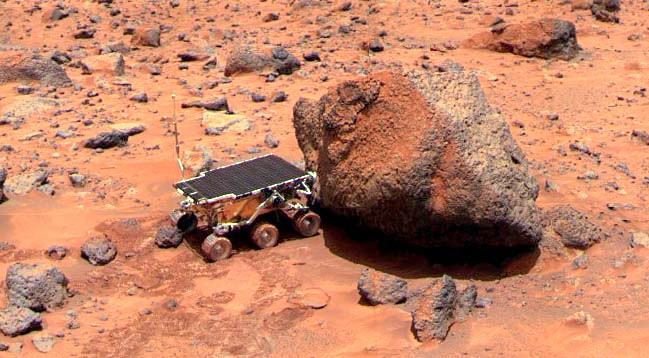
\includegraphics[height=2.5cm, width=4cm]{mars.jpg}
        \end{tabular}
        & \begin{tabular}{l}
            \parbox{0.5\linewidth}{
                After the Mars Pathfinder landed on Mars, VxWorks the real-time
                operating system began experiencing total system resets
                resulting in data loss. \\
                Priority inversion made the high-priority bus management task
                block on a mutex for bus access. This caused the system to
                periodically reboot the system. Luckily support of priority
                inheritance was present on the VxWorks kernel and by using a
                c-shell the team enabled this feature with a command sent from
                the earth.
            }
        \end{tabular}  \\
    \end{tabular}
\end{frame}

\begin{frame}
    \frametitle{Definition}
    Non blocking algoritms can be categorized into following classification.
    \begin{description}[Obstruction Freedom]
        \item[Obstruction Freedom] Means that we gurantee progress as long
            there is no contention between thread.
        \item[Lock Freedom] Adds the requirement that the system as a whole
            makes progress even if there is contention.
        \item[Wait Freedom] Adds the requirement that every thread makes
            progress even if meets contention.
    \end{description}
\end{frame}

\section{How to Achieve Lock Freedom}
\begin{frame}
    \frametitle{Tools and Features}
    There are a number of tools and features that hardwares and compilers
    provide us with in order to achieve lock freedom.
    \begin{itemize}
        \item Atomic Primitives
        \item Memory Models of Specific Architectures and how programming
            languages exploit them
    \end{itemize}
\end{frame}

\subsection{Atomic Primitives}
\begin{frame}
    \frametitle{Architecture Specific Atomic Primitives}
    To serialize the program order we need atomic primitives.
    Different Architectures present different methods for serializing the
    program order.
    \begin{itemize}
        \item Load-Linked \& Store-Conditional
        \item Fences
        \item Compare And Exchange
    \end{itemize}
\end{frame}

\subsection{Memory Models}
\begin{frame}
    \frametitle{Memory Models}
    Memory models define the interface between the programmer and the system.
    This model defines the ordering of externally visible events such as
    writes and reads to the memory system. \\
    This is important when we are trying to design or verify multi-threaded
    systems. \\
    An example of memory models are
    \begin{itemize}
        \item Sequencial Consistency
        \item Weak Ordering
    \end{itemize}
    But models are not limited to these most architectures have their own
    ordering That should be studied like the intel memory ordering paper.
\end{frame}

\subsection{C++ Memory Model}
\begin{frame}
    \frametitle{C++ Memory Model}
    memory\_order enum describes how the atomic functions should behave with
    regards to the memory model.
    \begin{itemize}
        \item seq\_qst: sequential consistency that we expect.
        \item consume: order the loads with loads and writes to the
            same address so that no loads or writes can happen before.
        \item acquire: order the loads with loads and writes to the
            any address so that no loads or writes can happen before.
        \item release: order the stores with loads and writes to the
            any address so that no loads or writes can happen before.
        \item acquire/release: sum of the two above
        \item relaxed: No memory ordering enforced.
    \end{itemize}

    One of the challenges in this section is how to use this model in formal
    methods more info can be found in  \cite{mckenney2017parallel}.
\end{frame}

\section{Lock-Free Algorithms}

\subsection{CAS Based Vector}
\begin{frame}
    \frametitle{CAS Based Vector}
    This vector was proposed by the \cite{dechev2006lock} and uses the compare
    and exchange atomic primitives to achieve lock freedom.
\end{frame}

\begin{frame}
    \frametitle{push\_back algorithm example}
    \begin{algorithmic}
        \Repeat
        \State $desc_{current} \gets vector.desc$
        \State $CompleteWrite(vector, desc_{current}.pending)$
        \If{$vector.memory[bucket]=NULL$}
        \State $AllocBucket(vector, bucket)$
        \EndIf
        \State $wop \gets new WriteDesc(At(desc_{current}.size)\^{}, elem,
        desc_{current}.size))$
        \State $desc_{next} \gets new Descriptor(desc_{current}.size + 1, wop)$
        \Until{$CAS(\&vector.desc, desc_{current}, desc_{next})$}
        \State $CompleteWrite(vector, desc_{next}.pending)$
    \end{algorithmic}
\end{frame}

\subsection{STM Based Vector}
\begin{frame}
    \frametitle{STM Based Vector}
    RSTM is a nonblocking stm algorithm that is described
    by \cite{marathe2006lowering}. Using this method the \cite{dechev2006lock}
    used algorithms presented by them to make another nonblocking vector
    container. \\
    STM based algorithms have too many features such as:
    \begin{itemize}
        \item Contention Management.
        \item Visible readers.
    \end{itemize}

\end{frame}

\begin{frame}
    \frametitle{push\_back algorithm example}
    \begin{algorithmic}
        \State $BEGIN\_TRANSACTION$
        \State sh\_ptr<STMVectorNode> nv = new sh\_ptr<STMVectorNode>(new
         STMVectorNode(v))
        \State sh\_ptr<STMVectorDesc> desc = new sh\_ptr\_<STMVectorDesc>
        (new STMVectorDesc($L_{desc}$ -> size + 1))
        \State mem[size] = nv
        \State $L_{desc} = desc$
        \State $END\_TRANSACTION$
    \end{algorithmic}
\end{frame}

\section{Results}
\begin{frame}
    \frametitle{Benchmarking Methods}
    All algorithms are implemented in the binary \textit{curious turtle}.
    At first the \textit{RDTSC} instruction was used to benchmark the
    selected code. \\
    This was wrong according to the intel manual that stated \textit{SMP}
    should be disabled.
    At last the the thread clock was used to get a measurement from the
    scheduler to benchmark this code.
\end{frame}

\begin{frame}
    \frametitle{clock\_gettime()}
    By tracing the \textit{clock\_gettime} syscall into the kernel we were able 
    to verify that the \textit{clock\_gettime} used with the \textit{CLOCK\_
    THREAD\_CPUTIME\_ID} returns the \textit{sum\_exec\_runtime} which is the
    bookkeeping information done by the scheduler. \\
    \textit{sum\_exec\_runtime} is updated by \textit{update\_curr} which is\
    called every time an interrupt or context switch occurs in the scheduler.
    The resolution of these clocks which the scheduler
    bases its calculation on in an intel-based system is
    governed by the \textit{tsc} which is run every 2903989 KHz on our system.
    This has been deemed as enough accuracy for us.
\end{frame}

\begin{frame}
    \frametitle{Results}
    \begin{figure}
        \centering
        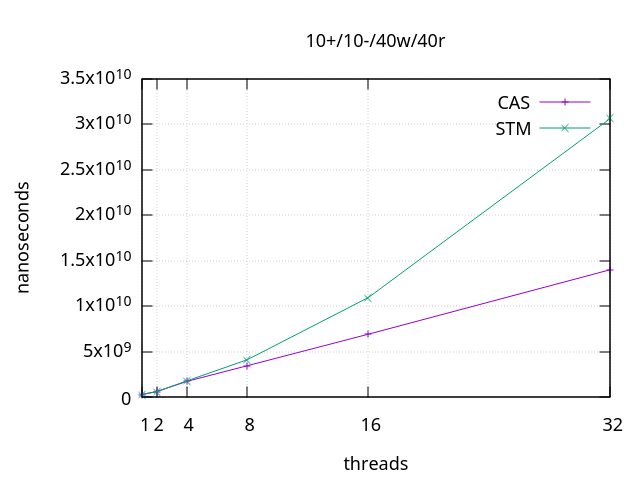
\includegraphics[width=0.7\textwidth]{results1.png}
        \caption{All threads results using 5 times warmup}
        \label{fig:res1}
    \end{figure}
\end{frame}

\begin{frame}
    \frametitle{Results}
    \begin{figure}
        \centering
        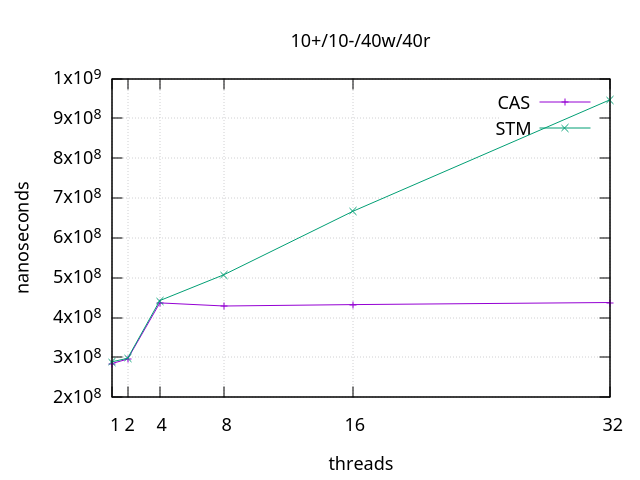
\includegraphics[width=0.7\textwidth]{results2.png}
        \caption{Per threads results using 5 times warmup}
        \label{fig:res2}
    \end{figure}
\end{frame}

\begin{frame}{Reference}
\bibliographystyle{apalike}
\bibliography{ref.bib} 
\end{frame}

\end{document}
